\documentclass[10pt,oneside,slovak,a4paper]{article}

\usepackage[slovak]{babel}
%\usepackage[T1]{fontenc}
\usepackage[IL2]{fontenc}
\usepackage[utf8]{inputenc}
\usepackage{graphicx}
\usepackage{url} % príkaz \url na formátovanie URL
\usepackage{hyperref} % odkazy v texte budú aktívne (pri niektorých triedach dokumentov spôsobuje posun textu)

\usepackage{cite}
%\usepackage{times}
%\usepackage{fancyhdr}
%\usepackage{csquotes} Uvodozvky    \enquote{TEXT}

%Nastavenie cesty pre obrazky
\graphicspath{ {./images/} }

\pagestyle{myheadings}%{headings} {fancy} zmiznu nazvy kapitol 
%\fancyhf{}
%\fancyhead[LE, RO]{\leftmark} LEFT EVEN, RIGHT ODD
%\fancyhead[RE, LO]{\thepage}
\title{Aplikácie a riešenia dištančného vzdelávania a e-vzdelávania\thanks{Semestrálny projekt v predmete Metódy inžinierskej práce, ak. rok 2020/21, vedenie: Ing. Fedor Lehocki, PhD.}}

\author{Lukáš Štrbo\\[2pt]
	{\small Slovenská technická univerzita v Bratislave}\\
	{\small Fakulta informatiky a informačných technológií}\\
	{\small \texttt{xstrbol@stuba.sk}}
	}

\date{\small 3. október 2020}



\begin{document}

\maketitle

\begin{abstract}
E-vzdelávanie sa stáva stále viac populárnejšou metódou nadobúdania vedomostí. Mnohí ľudia ju preferujú najmä kvôli rýchlosti a efektívnosti získavania poznatkov.
Prostredníctvom internetu sa dokážeme vzdelávať pomocou rôznych aplikácií, webov, kurzov alebo aj diskusných fór.
S e-vzdelávaním ide ruka v ruke dištančné vzdelávanie, ktoré hlavne v ťažších časoch, ako je napríklad nemožnosť zúčastňovať sa prezenčnej výučby z dôvodu pandémie COVID-19, 
 je voľbou číslo jedna. Rozdiely v medzi e-vzdelávaním a dištančným vzdelávním si rozoberieme v kapitole \ref{rozdiely}. Cieľom tejto práce je sprehľadniť čitateľovi rôzne metódy dištančného vzdelávania. Rozoberieme si a porovnáme riešenia dištančného vzdelávania a ich priamu
 aplikáciu. Zameriame sa na výhody a nevýhody, ale aj ktoré softvéry alebo platformy sú lepšie pre dištančné vzdelávanie v praxi. 
 V rámci porovnávania sa zameriame aj na efektivitu a aplikáciu daných metód dištančného vzdelávania.
\end{abstract}



\section*{Úvod} %Nezobrazi sa cislovanie
\label{uvod}
%Uvod do problematiky
Vzdelávanie sa prostredníctvom počítača a webu sa stáva stále viac populárnejšou a častejšou metódou výučby či sa jedná o školy alebo o samoukov. V súvislosti aj s celosvetovou pandémiou 
 COVID-19 bola väčšina škôl nútená prejsť na dištančné vzdelávanie. Pod dištančným vzdelávaním rozuemieme aj e-learning. Tieto výrazy si rozoberieme v kapitole\ref{rozdiely}.  

\section{Definícia dištančného vzdelávania a e-vzdelávania}
\label{rozdiely}
\subsection{Dištančné vzdelávanie}
Dištančné vzdelávanie je proces výučby, ktorý prebieha na diaľku bez priameho kontaktu učiteľa a študenta.\cite{India}. %ktorý predstavuje situáciu, kde sú študenti oddelení od učiteľov na diaľku
Dištančné vzdelávanie zahŕňa poskytovanie systémov (elektronických alebo iných) na nadviazanie a udržiavanie komunikácie medzi učiteľmi a študentmi.
Stará koncepcia dištančného vzdelávania bola spojená výlučne s tlačenými materiálmi, zatiaľ čo nová koncepcia dištančného vzdelávania zahŕňa doplnkový materiál používaný prostredníctvom netlačených médií, ako je rozhlas, televízia, počítače, notebooky, nahrané prednášky vo formáte videí, prostredníctvom projektorov, videokonferencií a interaktívnych stretnutí medzi študentmi.

Existujú 2 typy dištančného vzdelávania, na základe interakcie študentov, a to synchrónne a asynchrónne dištančné vzdelávanie. %Bez ciarok povodne
Synchrónna metóda vyžaduje prezenčnú účasť študenta takzvane tvárou v tvár. %Interakcia sa uskutočňuje v „reálnom čase“ a je bezprostredná. %tzv. -> takzvane 
Asynchrónna metóda nevyžaduje prezenčnú účasť.
Potreba, aby sa študenti a učitelia zhromaždili prezenčne, je vylúčená a študenti si sami zvolia vlastný časový rámec na interakciu. %na stretnutí -> prezenčne
\subsection{E-vzdelávanie}
E-vzdelávanie je prirodzene vhodné na dištančné a flexibilné vzdelávanie, ale dá sa použiť aj v spojení s prezenčnou výučbou \cite{elearningDef}. %tzv. takzvane, takzvane tvárou v tvár
V prípade spojenia s prezenčnou výučbou sa používa termín Blended learning. %V takom prípade sa bežne používa termín Blended learning. 
E-vzdelávanie môže tiež odkazovať na vzdelávacie webové stránky, ako napríklad webové stránky ponúkajúce pracovné listy a interaktívne cvičenia.
Výraz e-vzdelávanie sa široko používa aj v obchodnom sektore, kde sa všeobecne vzťahuje na nákladovo efektívne on-line školenia.
E-vzdelávanie je závislé od technológii, podporuje a zlepšuje výučbu.
So zameraním na používanie internetu v e-vzdelávaní, sa objavili tri hlavné spôsoby použitia.
Ide o elektronickú technológiu na poskytovanie, podporu a zdokonaľovanie výučby a učenia sa. 

\section{Typy dištančnej výučby}
%Uvod do typov distancnej vyucby
Dištančnou výučbu rozdeľujeme na nasledujúce typy\cite{WiktorzakKotowski}:
\begin{itemize}
	\item \textbf{Technology-based training (TBT)} alebo aj e-vzdelávenie. %je totožné s e-vzdelávaním.
	\item \textbf{Computer-based trainig (CBT)}, ktorý používa počítače vo výučbovom procese na prenos znalostí, vykonávanie cvičení alebo simulácii. V rámci tohto konceptu sú aj rôzne kurzy, ktoré v minulosti boli dodávané na CD.
	\item \textbf{Web-based training (WBT)} je typ dištančnej výučby, ktorý prebieha na internete prostredníctvom protokola TCP/IP. Zahŕňa prenos znalostí ako aj ich overenie, komunikáciu medzi používateľmi a riadením vzdelávacieho procesu s využitím webových stránok a webových aplikácií.
\end{itemize}

Vyššie spomenuté typy dištančnej výučby sú spojené s použítím špecifických technológií. 
Avšak najviac používaný edukačný model kombinuje počítačovú technológiu s prezenčnou výučbou.%tradičným spôsobom vedenia tried na univerzitách.

V dôsledku toho rozlišujeme dištančnú výučbu na :
\begin{itemize}
	\item \textbf{Instructor-led training (ILT)} je výučbový proces, v ktorom učiteľ vyučuje skupinu študentov. Hodiny prebiehajú väčšinou priamo v priestoroch školy. Tradičná výučba môže nadobudnúť aj takú formu, počas ktorej učiteľ komunikuje so žiakmi prostredníctvom internetu.
	\item \textbf{Synchronous learning (SL)} znamená, že aktivity a výučba sú vedené v reálnom čase, ale sú realizované cez internet. Študenti aj učitelia sú prihlásení do jedného systému, takzvaného virtuálneho učebného priestoru, v ktorom prebieha výučba.
	\item \textbf{Blended learning (BL)} alebo aj hybridné vyučovanie je spôsob výučby, ktorý kombinuje tradičný model výučby s dištančnou formou výučby. V tomto modeli výučby sú prednášky prednášané väčšinou vzdialene a prebiehajú on-line konzultácie, zatiaľ čo cvičenia a praktické hodiny sa uskutočňujú priamo na univerzite prezenčnou formou.
\end{itemize}


\begin{figure}[h]
	\centering
	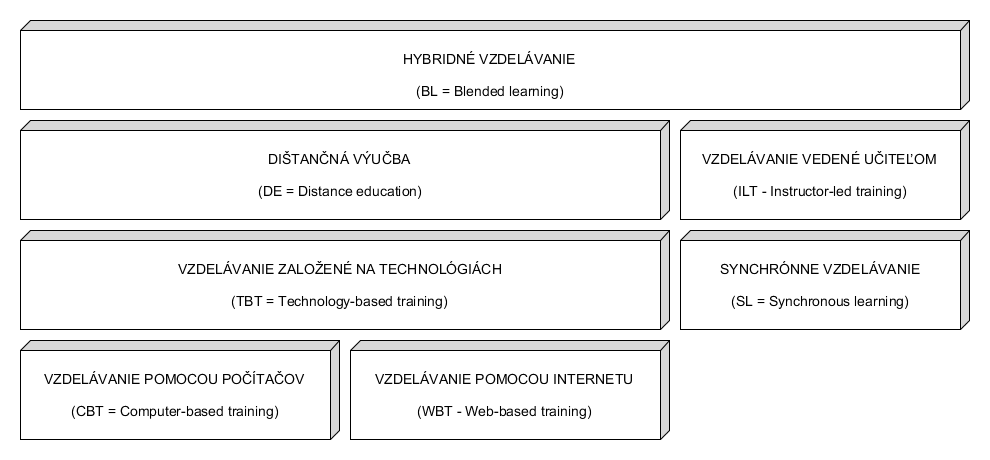
\includegraphics[width=\textwidth]{Vztahy_DE.png}
	\caption{Vzťahy medzi pojmami v dištančnom vzdelávaní\cite{WiktorzakKotowski}}
	\label{Vztahy_medzi_pojmami}
\end{figure}

%Referencia na obrazok
Vzťahy medzi pojmami spojenými s dištančným vzdelávaním sú znázornené na obrázku \ref{Vztahy_medzi_pojmami}.%obrazok 1 alebo obrazok Č. 1
Oblasť dištančného vzdelávania pokrýva širokú sféru technológií a metód vzdelávania. %oblast technologii / %Je to okrem iného spôsobené potrebou neustálej odbornej prípravy v čoraz viacerých oblastiach.
V závislosti od prenášaného obsahu (napr. kurz v angličtine), sa používajú rôzne nástroje a techniky výučby.
%V nasledujúcej časti nájdete stručný popis nástrojov dištančného vzdelávania.

\section{Vývoj podporných systémov pre dištančné vzdelávanie}%ALEBO : Podporne systemy pre distancne vzdelavanie
\label{Vyvojsys}
Systémy podporujúce dištančné vzdelávanie boli pôvodne navrhnuté na výučbu pomocou počítača (CBT)\cite{WiktorzakKotowski}.%Tieto systémy sa neustále rozvíjajú.

S príchodom internetu sa objavilo veľa nástrojov, ktoré podporujú vzdelávanie prostredníctvom webu (WBT).
Pôvodne išlo len o statické stránky, ktoré poskytovali učebné materiály.
Neskôr sa objavili dynamické stránky, ktoré vyžadovali určitú interakciu používateľov, ako sú napríklad diskusné fóra alebo interaktívne cvičenia.
Ide o internetové služby, ktoré spolupracujú s databázou obsahujúcou učebné materiály a testy na kontrolu vedomostí študentov. %a tiež obsahu zadaného používateľmi.
Takéto služby umožňujú učenie a komunikáciu v asynchrónnom režime. Učebné materiály môže učiteľ priebežne aktualizovať a ukladať do elektronickej databázy.
Priama komunikácia medzi študentom a učiteľom je nadviazaná aj vďaka e-mailu.

Ďalším krokom vo vývoji systémov na podporu dištančného vzdelávania bol vznik synchrónnych komunikačných nástrojov, ako sú chat, audio a videokonferencie, virtuálna tabuľa a zdieľanie obrazovky.
Spojenie týchto komunikačných nástrojov do aplikácie funguje ako virtuálna učebňa.
Dnes sú to napríklad Google Classroom, Google Meet, Cisco Webex Meetings, Zoom Meetings, Microsoft Teams a podobne.
Vývoj podporných systémov je zobrazený na obrázku \ref{Vyvoj_podp_sys_DE}.

\begin{figure}[]
	\centering
	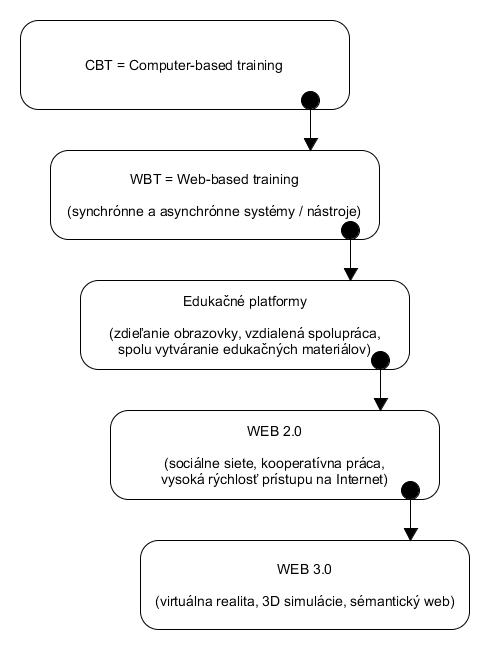
\includegraphics[scale=0.15, height=100mm,width=0.6\textwidth]{Dev_Of_SupSys_DE.jpg}
	\caption{Vývoj podporných systémov pre dištančné vzdelávanie\cite{WiktorzakKotowski}}
	\label{Vyvoj_podp_sys_DE}
\end{figure}

%\subsection{Najviac používané}
%Webex, Meet, MS TEAMS, porovnanie , obluba u studentov, vlastnosti
%\subsection{Edukačné platformy}
%Edukacne platformy - Online testovanie , Edupage, AIS, Kurzy online, Moodle, ...
\section{Výzvy vo vzdelávaní počas pandémie COVID-19}
\subsection{Výučba počas pándémie COVID-19} %TOTO BOLA PREDTYM SEKCIA
V súvislosti s pandémiou COVID-19 boli školy a univerzity zatvorené a pre zabezpečenie kontinuity vzdelávania, sa z prezenčnej výučby prešlo na on-line výučbu \cite{covid19}.
Sme tak svedkami núteného prerušenia klasickej organizácie vzdelávania, jej štruktúr a rutín. Prioritou všetkých vzdelávacích systémov je neprerušovať výučbu.
Preto sa pokladá za dôležité zabezpečiť výučbu aj v on-line priestore a zabezpečiť dôsledné spojenie medzi učiteľmi a žiakmi. 

Medzi rôzne iniciatívy na oslovenie študentov počas on-line výučby, patrí:  %ktoré uprednostňujú vlády, školy alebo učitelia s cieľom efektívne 
\begin{itemize}
	%\item Vypracovanie podporných dokumentov, ako sú metodiky, príručky, balíčky zdrojov pre presun výučby v on-line prostredí.
	\item Využívanie špecializovaných platforiem pre on-line výučbu a oficiálnych webových stránok, ktoré centralizujú iniciatívy v tejto oblasti\ref{Vyvojsys}.%KONTROLA !!!!
	\item Podpora študentov a rodičov prostredníctvom častých správ, vysvetlení, otázok a odpovedí za pomoci používania e-mailov a sociálnych sietí.
	\item Reorganizácia hodnotiacich postupov, ako napríklad úprava alebo zrušenie skúšok, písomiek a testov.
	\item Zavedenie konkrétnych opatrení zameraných na dosiahnutie rovnosti vo vzdelávaní, najmä preto, že zraniteľné skupiny sa počas krízových situácií stávajú ešte viac zraniteľnejšími (príkladom je poskytnutie počítačov a telekomunikačných balíkov úradmi pre rodiny v ťažkostiach).
\end{itemize}

\subsection{Výskum}%NAZOV ????
\subsubsection{Zámer výskumu}
Zámerom výskumu bolo zistiť\cite{covid19}:
\begin{enumerate}
	\item Aké sú najčastejšie používané on-line riešenia.
	\item Či bol alebo nebol adaptačný proces na tento nový typ didaktickej činnosti náročný a aké prekážky v ňom boli.
	\item Výhody a nevýhody on-line prostredia vo vzdelávacom kontexte.
	\item Najväčšie obavy študentov týkajúce sa vzdelávacích aktivít. %, keď sa blížia ku koncu školského roka
\end{enumerate}
\subsubsection{Vzorka a nástroje výskumu}
Vzorku vo výskume tvorilo 152 študentov z Fakulty psychológie a pedagogických vied Ovídiovej univerzity v Konstanci, ktorá sa nachádza v Rumunsku \cite{covid19}.
Zúčastnení výskumu boli ženy vo veku od 18 do 52 rokov zo všetkých stupňov štúdia.
Výskum sa uskutočnil on-line pomocou Google formulárov. %Anketa pozostávala z 8 otázok s konkrétnymi odpoveďami, z ktorých si účastníci mohli vybrať jednu alebo viac odpovedí. 
%Vyskum bol tvoreny z 8mich otazok, ale v tomto dokumente si rozoberieme iba 4 z nich.
\subsection{Výsledky výskumu}%ESTE NEOPRAVENE TEXTY
Vo výskume boli zistené nasledujúce výsledky\cite{covid19} : % zistenia a
\begin{itemize}
	
	\item Prvá otázka sa opýtala účastníkov na ich názor ohľadom prechodu z prezenčnej výučby na dištančnú výučbu spôsobeného pandémiou COVID-19. 64.47\% opýtaných odpovedalo, že im vyhovuje dištančná výučba. Pre 34,21\% opýtaných je dištančná výučba prijateľná a pre 1,31\% opýtaných dištančná výučba je neprijateľná a nevyhovuje im.
	\item Druhá otázka sa opýtala účastníkov, aby vymenovali najpoužívanejšie on-line platformy počas dištančného vzdelávania. Výsledky ukazujú, že 92,10\% účastníkov a ich učiteľov používa Cisco Webex Meetings, 42,10\% používa WhatsApp a e-mail, 41,44\% Zoom Meetings, 1,31\% Moodle a 1,31\% Academis.
	\item Tretia otázka položila účastníkom otázku, či bol proces adaptácie na dištančné vzdelávanie problematický alebo nie. 76,97\% študentov nemalo ťažkosti s adaptáciou na nový typ vzdelávania, zatiaľ čo 22,36\% študentov malo problémy s adaptáciou.
	%\item  DOROBIT OTAZKY
\end{itemize}



\section{Výhody a nevýhody dištančnej výučby}
V nasledujúcich podkapitolách si rozoberieme výhody a nevýhody dištančného vzdelávania\cite{Sokolova2018}. 
\subsection{Výhody}
\begin{itemize}
	\item Pre študovanie na diaľku študent potrebuje zariadenie s prístupom na internet, ako napríklad počítač, tablet alebo smartfón. Študent sa sám rozhodne, kedy a kde bude učebné materiály študovať.
	\item Vďaka možnosti študovať na diaľku je možné napríklad ušetriť peniaze za školné, dopravu a tiež ubytovanie pre študentov. Študenti tiež nemusia platiť za učebnice, skriptá a ďalšiu literatúru.
	\item Ďalšou z výhod je, že ak niektorí študenti niečo nepochopili, nie vždy sa odvážia položiť otázku učiteľovi, ale v rámci dištančného vzdelávania, sa nesmelí študenti cítia komfortnejšie v kladení otázok. 
	\item Študenti si môžu prednášku vypočuť viackrát.%, ktorí potrebujú viac času na premýšľanie o informáciách ako ich spolužiaci, si zároveň môžu prednášku vypočuť viackrát, dlhšie sa zamýšľajú nad poskytnutým materiálom a potom, ak ešte niečo zostane nezrozumiteľné, opýtajú sa lektora.
	\item Dištančné vzdelávanie umožňuje učiteľom rýchlo získať spätnú väzbu od veľkého počtu študentov. Vzdelávanie prebieha interaktívnou formou. Každý študent má možnosť klásť učiteľovi otázky, ktoré ho zaujímajú. Študent môže diskutovať nielen so samotným učiteľom, ale aj s ostatnými poslucháčmi.
	\item Ďalšou pozitívnou vlastnosťou dištančného vzdelávania je, že je ideálnou alternatívou denného štúdia pre ľudí so zdravotným postihnutím. Títo študenti nemajú vždy majú fyzicky navštevovať hodiny z dôvodu zlého zdravotného stavu. Niektorí z nich potrebujú špeciálne vybavené rampy pre invalidné vozíky, čo pre univerzitu predstavuje problém s vytváraním špeciálnych zariadení a zvyšuje náklady na údržbu a vybavenie priestorov.
\end{itemize}
\subsection{Nevýhody}
\begin{itemize}
	\item Študent je zbavený živej komunikácie s učiteľom aj s ostatnými študentmi. Prednášky tým strácajú veľa na významovom obsahu.
	\item Ďalším negatívnym aspektom dištančného vzdelávania je skutočnosť, že nesmelí študenti, ktorí sa cítia lepšie pri interakcii na diaľku, si nezvyknú na živú komunikáciu.
	\item Testovací systém je veľmi vhodný na on-line hodnotenie, ale nie je vhodný na rozvoj schopnosti samostatne myslieť, asimilovať materiál a snažiť sa ho uplatniť vo svojom živote. Výsledky, ktoré získa študent po zvládnutí daného testu, nebudú vždy odrážať úroveň jeho vedomostí z témy, na ktorú sa pripravoval.
	\item Dlhodobá práca na počítači má negatívny vplyv na zdravie, zrak a chrbticu.
\end{itemize}



%\section{Aplikácia dištančnej výučby v praxi}
%\subsection{Základné a stredné školy}
%\subsection{Vysoké školy}
%\subsection{Virtuálne univerzity}

%\section{Efektivita a dopad dištančnej výučby}
%\subsection{Efektívnosť}
%\subsection{Výhody a nevýhody}


%\acknowledgement{Ak niekomu chcete poďakovať\ldots}



\bibliography{zdroje}
\bibliographystyle{plain}
\end{document}
